% Type of the document
\documentclass{beamer}

% elementary packages:
\usepackage{graphicx}
\usepackage[latin1]{inputenc}
\usepackage[T1]{fontenc}
\usepackage[english]{babel}
\usepackage{listings}
\usepackage{xcolor}
\usepackage{eso-pic}
\usepackage{mathrsfs}
\usepackage{url}
\usepackage{amssymb}
\usepackage{amsmath}
\usepackage{multirow}
\usepackage{hyperref}
\usepackage{booktabs}
\usepackage{tikz}

% additional packages
\usepackage{bbm}

% packages supplied with ise-beamer:
\usepackage{cooltooltips}
\usepackage{colordef}
\usepackage{beamerdefs}
\usepackage{lvblisting}

% Change the pictures here:
% logobig and logosmall are the internal names for the pictures: do not modify them. 
% Pictures must be supplied as JPEG, PNG or, to be preferred, PDF
\pgfdeclareimage[height=2cm]{logobig}{hulogo}
% Supply the correct logo for your class and change the file name to "logo". The logo will appear in the lower
% right corner:
\pgfdeclareimage[height=0.7cm]{logosmall}{Figures/LOB_Logo}

% Title page outline:
% use this number to modify the scaling of the headline on title page
\renewcommand{\titlescale}{1.0}
% the title page has two columns, the following two values determine the percentage each one should get
\renewcommand{\titlescale}{1.0}
\renewcommand{\leftcol}{0.6}

% Define the title.Don't forget to insert an abbreviation instead 
% of "title for footer". It will appear in the lower left corner:
\title{Analyzing the Ringelmann Effect with the Repeated Measures ANOVA }
% Define the authors:
\authora{Nikolas H�ft\\
	Constantin Meyer-Grant\\
	Joachim Munch\\
	Quang Nguyen Duc\\
	Frederik Schreck} % a-c


% Define any internet addresses, if you want to display them on the title page:
\def\linkb{}
\def\linkc{}
% Define the institute:
\institute{Statistical Programming Languages\\
	Humboldt-Universit�t zu Berlin}

% Comment the following command, if you don't want, that the pdf file starts in full screen mode:
\hypersetup{pdfpagemode=FullScreen}

%Start of the document
\begin{document}

% create the title slide, layout controlled in beamerdefs.sty and the foregoing specifications
\frame[plain]{
	\titlepage
	}

% The titles of the different sections of you talk, can be included via the \section command. The title will be displayed in the upper left corner. To indicate a new section, repeat the \section command with, of course, another section title
%%%%%%%%%%%%%%%%%%%%%%%%%%%%%%%%%%%%%%%%%%%%%%%%%%%%%%%%%%%%%%%%%%%%%%%%%%%%%%%%%%%%%%%%%%%%%%%%%%%%%%%%%%%%%%%%%%%%%%%%
\section{Introduction}
%%%%%%%%%%%%%%%%%%%%%%%%%%%%%%%%%%%%%%%%%%%%%%%%%%%%%%%%%%%%%%%%%%%%%%%%%%%%%%%%%%%%%%%%%%%%%%%%%%%%%%%%%%%%%%%%%%%%%%%%

% (A numbering of the slides can be useful for corrections, especially if you are
% dealing with large tex-files)

%%%%%%%%%%%%%%%%%%%%%%%%%%%%%%%%%%%%%%%%%%%%%%%%%%%%%%%%%%%%%%%%%%%%%%%%%%%%%%%%%%%%%%%%%%%%%%%%%%%%%%%%%%%%%%%%%%%%%%%%
\section{}
\useheadtemplate{%
	\raisebox{-0.75cm}{\parbox{\textwidth}{%
			\footnotesize{\color{isegrey}%
				\insertsection\ \leavevmode\leaders\hrule heigth3.2pt depth-2.8pt\hfill\kern0pt\}}}
		}

\frame{
	\frametitle{Outline}
	\begin{enumerate}
		\item The Ringelmann Effect
		\item Repeated Measures ANOVA
		\begin{enumerate}
			\item The ANOVA model
			\item An Advantageous Model
			\item Confidence Intervals
			\item Effect Size
		\end{enumerate}
		\item An Important Requirement
		\item Orthogonal Polynomial Contrasts
		\item The Package
	\end{enumerate}
}

\useheadtemplate{%
	\raisebox{-0.75cm}{\parbox{\textwidth}{%
			\footnotesize{\color{isegreq}%
				\insertsection\ \leavevmode\leaders\hrule height3.2pt depth-2.8pt\hfill\kern0pt\ \thesection-\thepage}}}}
\setcounter{section}{1}
			
%%%%%%%%%%%%%%%%%%%%%%%%%%%%%%%%%%%%%%%%%%%%%%%%%%%%%%%%%%%%%%%%%%%%%%%%%%%%%%%%%%%%%%%%%%%%%%%%%%%%%%%%%%%%%%%%%%%%%%%%
\frame[containsverbatim]{
	\frametitle{The Ringelmann Effect}
	\begin{itemize}
	\item Maximilian Ringelmann (1861-1931):
	 \begin{itemize}
	 \item French professor of agricultural ingeneering
	 \end{itemize}
	\item Work performance depends of number of group size
	\item Decreasing individual performance with increasing group size 
	\item Example: Pulling weights with different sized groups
	\end{enumerate}
}


%%%%%%%%%%%%%%%%%%%%%%%%%%%%%%%%%%%%%%%%%%%%%%%%%%%%%%%%%%%%%%%%%%%%%%%%%%%%%%%%%%%%%%%%%%%%%%%%%%%%%%%%%%%%%%%%%%%%%%%%
\frame[containsverbatim]{
	\frametitle{The Ringelmann Effect}
	\begin{itemize}
		\item The Ringelmann Effect can be investigated with an experimental design
		\begin{itemize}
			\item Dependent Variable: Indivual performance
			\item Independent Variable / Factor: Group size 
			\item Realization of different factor levels
		\end{itemize}
		\item For our purpose: Data simulation \quantnet Quantlet Data Simulation
	\end{enumerate}
}


%%%%%%%%%%%%%%%%%%%%%%%%%%%%%%%%%%%%%%%%%%%%%%%%%%%%%%%%%%%%%%%%%%%%%%%%%%%%%%%%%%%%%%%%%%%%%%%%%%%%%%%%%%%%%%%%%%%%%%%%
\frame[containsverbatim]{
	\frametitle{The Ringelmann Effect}
	\begin{itemize}
	\item The Ringelmann Effect can be investigated with an experimental design
	\begin{itemize}
	\item Dependent Variable: Indivual performance
	\item Independent Variable / Factor: Group size 
	\item Realization of different factor levels
	\end{itemize}
	\item For our purpose: Data simulation \quantnet Quantlet Data Simulation
	\end{enumerate}
}

%%%%%%%%%%%%%%%%%%%%%%%%%%%%%%%%%%%%%%%%%%%%%%%%%%%%%%%%%%%%%%%%%%%%%%%%%%%%%%%%%%%%%%%%%%%%%%%%%%%%%%%%%%%%%%%%%%%%%%%%

\frame[containsverbatim]{
	\frametitle{Code}
}	
	
	
%%%%%%%%%%%%%%%%%%%%%%%%%%%%%%%%%%%%%%%%%%%%%%%%%%%%%%%%%%%%%%%%%%%%%%%%%%%%%%%%%%%%%%%%%%%%%%%%%%%%%%%%%%%%%%%%%%%%%%%%
	
\frame[containsverbatim]{
	\frametitle{The Ringelmann Effect} %% Insert Data Graphic!
	\begin{figure}[htb]
	\begin{center}
	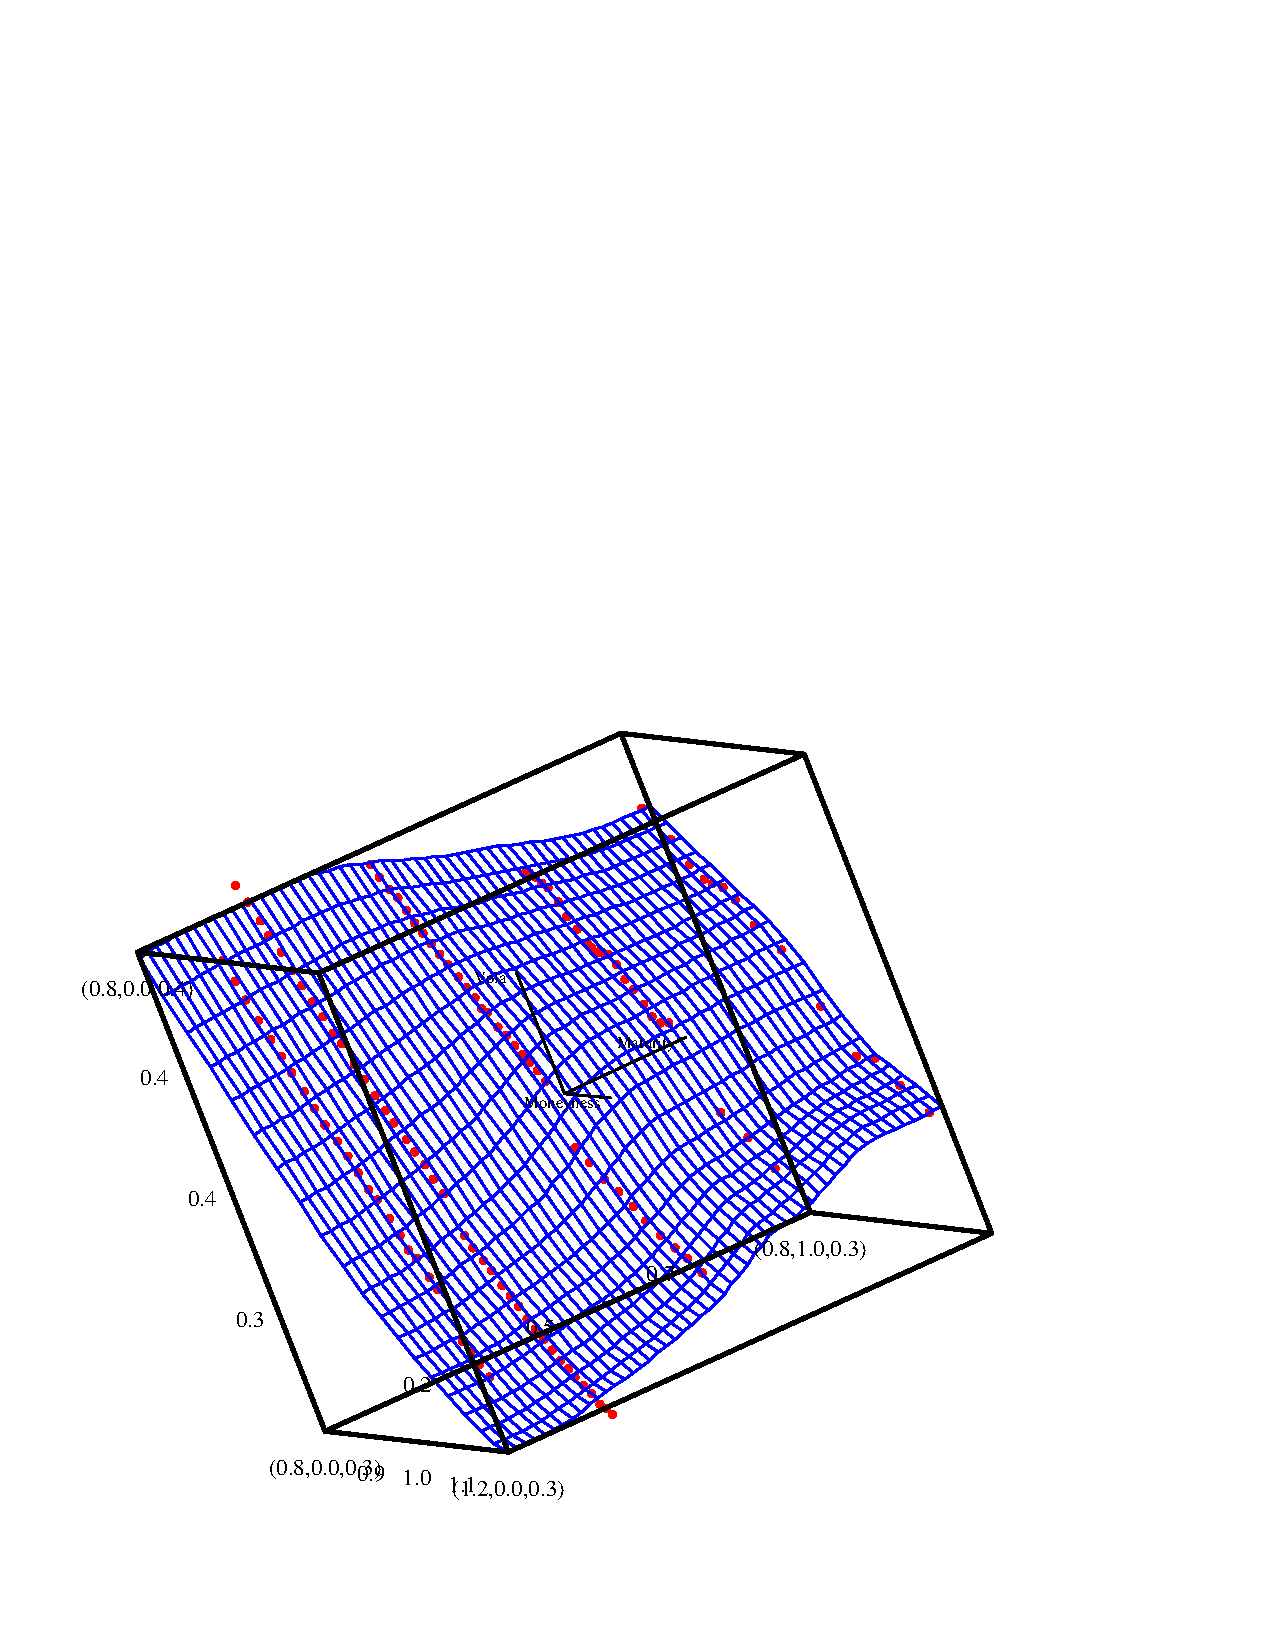
\includegraphics[scale=0.2]{Figures/vola}
	\caption{Include a short, but meaningful caption.}
	\end{center}
	\end{figure}
}

%%%%%%%%%%%%%%%%%%%%%%%%%%%%%%%%%%%%%%%%%%%%%%%%%%%%%%%%%%%%%%%%%%%%%%%%%%%%%%%%%%%%%%%%%%%%%%%%%%%%%%%%%%%%%%%%%%%%%%%%
\frame[containsverbatim]{
	\frametitle{The Repeated Measures ANOVA:  The ANOVA model} 
	\begin{itemize}
	\item ANOVA: Analysis of Variance
	\item Comparison of the \textit{k} factor level means
		\begin{eqnarray*}
		H_{0}: {\mu_{1}} = {\mu_{2}} = ... = {\mu_{k}} 
		\end{eqnarray*}
		\begin{eqnarray*}
		H_{1}: \exists i \not= j: {\mu_{i}} \not= {\mu_{j}} 
		\end{eqnarray*} 
		\\
	\item Test is accomplished by decomposition of variance components
	\end{enumerate}
}

%%%%%%%%%%%%%%%%%%%%%%%%%%%%%%%%%%%%%%%%%%%%%%%%%%%%%%%%%%%%%%%%%%%%%%%%%%%%%%%%%%%%%%%%%%%%%%%%%%%%%%%%%%%%%%%%%%%%%%%%

\frame[containsverbatim]{
	\frametitle{Code}
}
	
	
%%%%%%%%%%%%%%%%%%%%%%%%%%%%%%%%%%%%%%%%%%%%%%%%%%%%%%%%%%%%%%%%%%%%%%%%%%%%%%%%%%%%%%%%%%%%%%%%%%%%%%%%%%%%%%%%%%%%%%%%

\frame[containsverbatim]{
	\frametitle{The Repeated Measures ANOVA: An Advantegeous Model}
		\begin{itemize}
		\item Problem: In case of large variance between different subjects\\
		\begin{itemize}
		$\Rightarrow$ High error variance
		$\Rightarrow$ Loss of power in F-Test
		\end{itemize}
		\item Repeated Measures ANOVA considers the between subject variance separately
		\begin{itemize}
		$\Rightarrow$ Relatively low error variance
		$\Rightarrow$ Gain of power in F-Test
		\end{itemize}
		\quantnet Reduction of error variance
		\end{itemize}
		\end{enumerate}
}
%%%%%%%%%%%%%%%%%%%%%%%%%%%%%%%%%%%%%%%%%%%%%%%%%%%%%%%%%%%%%%%%%%%%%%%%%%%%%%%%%%%%%%%%%%%%%%%%%%%%%%%%%%%%%%%%%%%%%%%%

	\frame[containsverbatim]{
		\frametitle{The Repeated Measures ANOVA: An Advantegeous Model} %% Insert SSE Pie chart Graphic!
		\begin{figure}[htb]
		\begin{center}
		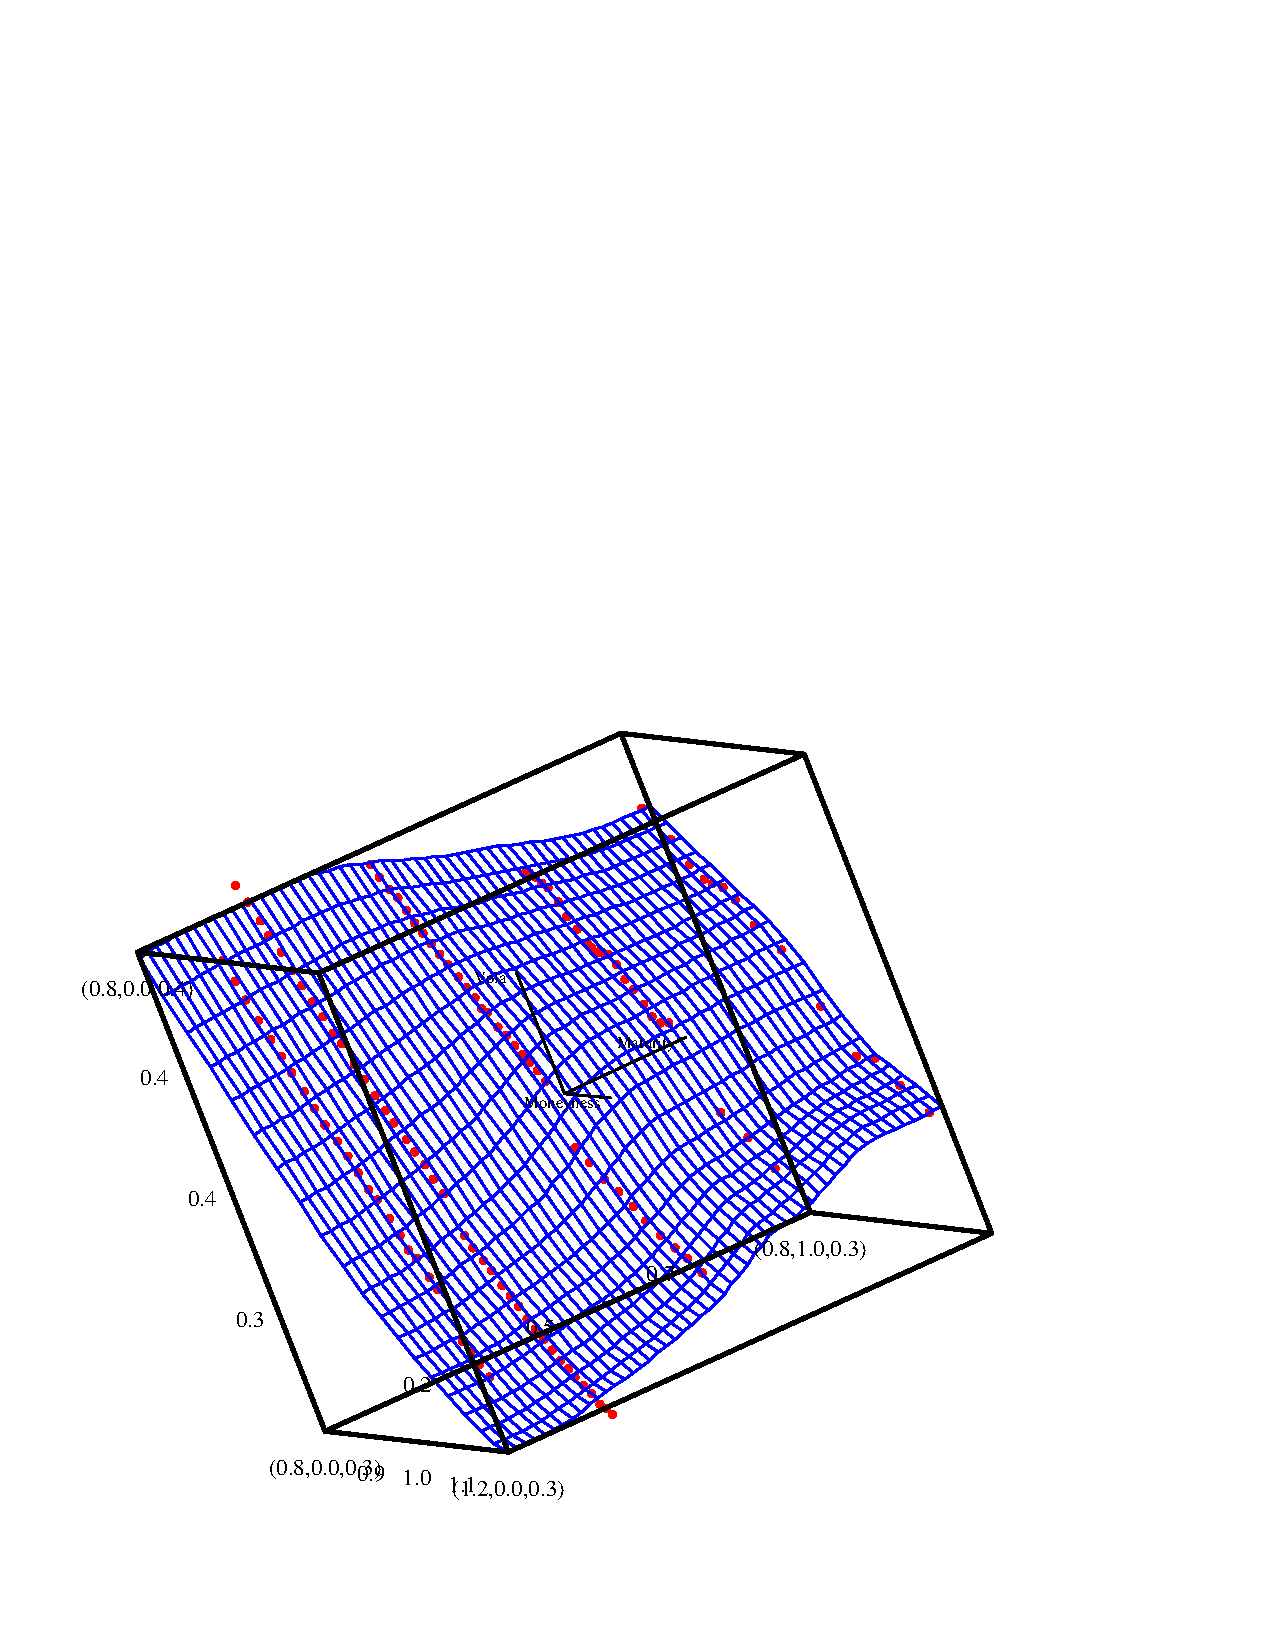
\includegraphics[scale=0.2]{Figures/vola}
		\caption{Include a short, but meaningful caption.}
		\end{center}
		\end{figure}
	}
	
%%%%%%%%%%%%%%%%%%%%%%%%%%%%%%%%%%%%%%%%%%%%%%%%%%%%%%%%%%%%%%%%%%%%%%%%%%%%%%%%%%%%%%%%%%%%%%%%%%%%%%%%%%%%%%%%%%%%%%%%

	\frame[containsverbatim]{
		\frametitle{The Repeated Measures ANOVA: An Advantegeous Model}
		\begin{itemize}
		\item Design Requirement: Each subject hast to be measured under all factor levels
		\begin{table}
		\begin{center}
		\begin{tabular}{cc} 
		\hline\hline
		Title & Title\\ 
		\hline
		2.13 & 1.45 \\
		3.14 & 6.85 \\
		\hline\hline
		\end{tabular}
		\caption{Example Data Matrix}
		\end{center}
		\end{table}
		\end{itemize}
	  	\end{enumerate}
	  }
	  	
	
%%%%%%%%%%%%%%%%%%%%%%%%%%%%%%%%%%%%%%%%%%%%%%%%%%%%%%%%%%%%%%%%%%%%%%%%%%%%%%%%%%%%%%%%%%%%%%%%%%%%%%%%%%%%%%%%%%%%%%%%

\frame[containsverbatim]{
	\frametitle{Code}

	
}

%%%%%%%%%%%%%%%%%%%%%%%%%%%%%%%%%%%%%%%%%%%%%%%%%%%%%%%%%%%%%%%%%%%%%%%%%%%%%%%%%%%%%%%%%%%%%%%%%%%%%%%%%%%%%%%%%%%%%%%%


\frame[containsverbatim]{
	\frametitle{Table}
	
	
}

%%%%%%%%%%%%%%%%%%%%%%%%%%%%%%%%%%%%%%%%%%%%%%%%%%%%%%%%%%%%%%%%%%%%%%%%%%%%%%%%%%%%%%%%%%%%%%%%%%%%%%%%%%%%%%%%%%%%%%%%

\frame[containsverbatim]{
	\frametitle{The Repeated Measures ANOVA: Confidence Intervals}
	\begin{itemize}
	\item The computation of the confidence intervals has to be adjusted in the Repeated Measures ANOVA
	\quantnet Confidence Intervals
	%% insert code
	\end{itemize}
	\end{enumerate}
}

%%%%%%%%%%%%%%%%%%%%%%%%%%%%%%%%%%%%%%%%%%%%%%%%%%%%%%%%%%%%%%%%%%%%%%%%%%%%%%%%%%%%%%%%%%%%%%%%%%%%%%%%%%%%%%%%%%%%%%%%

\frame[containsverbatim]{
	\frametitle{Code}
	
	
}

%%%%%%%%%%%%%%%%%%%%%%%%%%%%%%%%%%%%%%%%%%%%%%%%%%%%%%%%%%%%%%%%%%%%%%%%%%%%%%%%%%%%%%%%%%%%%%%%%%%%%%%%%%%%%%%%%%%%%%%%

	\frame[containsverbatim]{
		\frametitle{The Repeated Measures ANOVA: Confidence Intervals} %% Insert confidence interval figure
		\begin{figure}[htb]
		\begin{center}
		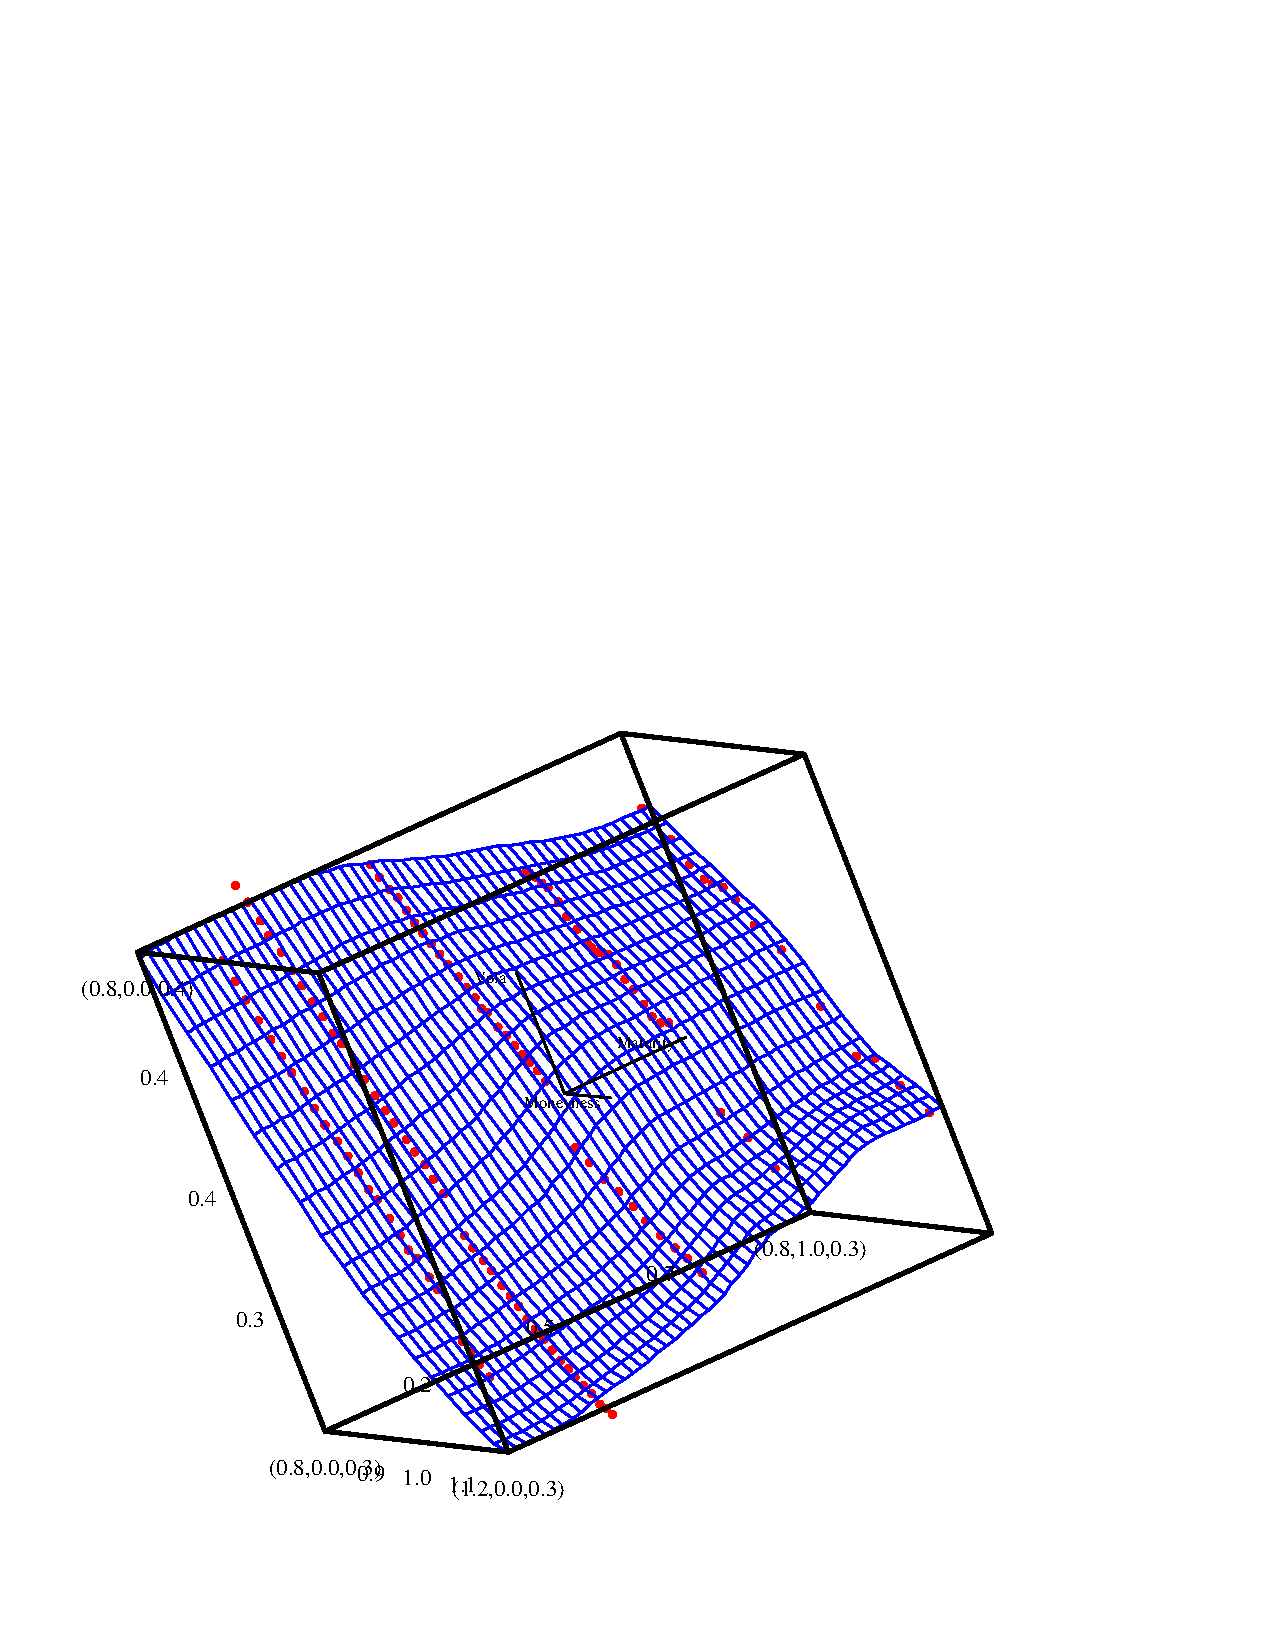
\includegraphics[scale=0.2]{Figures/vola}
		\caption{Include a short, but meaningful caption.}
		\end{center}
		\end{figure}
	}
	
%%%%%%%%%%%%%%%%%%%%%%%%%%%%%%%%%%%%%%%%%%%%%%%%%%%%%%%%%%%%%%%%%%%%%%%%%%%%%%%%%%%%%%%%%%%%%%%%%%%%%%%%%%%%%%%%%%%%%%%%

\frame[containsverbatim]{
	\frametitle{The Repeated Measures ANOVA: Effect Size Measures}
	\begin{itemize}
	\item Two measures of effect size: 
	\begin{itemize}
	\item $\eta^2$
	\item $\eta_{p}^2$
	\end{itemize}
	\end{itemize}
	\end{enumerate}
}

%%%%%%%%%%%%%%%%%%%%%%%%%%%%%%%%%%%%%%%%%%%%%%%%%%%%%%%%%%%%%%%%%%%%%%%%%%%%%%%%%%%%%%%%%%%%%%%%%%%%%%%%%%%%%%%%%%%%%%%%

\frame[containsverbatim]{
	\frametitle{Code}
	
	
}

%%%%%%%%%%%%%%%%%%%%%%%%%%%%%%%%%%%%%%%%%%%%%%%%%%%%%%%%%%%%%%%%%%%%%%%%%%%%%%%%%%%%%%%%%%%%%%%%%%%%%%%%%%%%%%%%%%%%%%%%

\frame[containsverbatim]{
	\frametitle{Table}
	
	
}

%%%%%%%%%%%%%%%%%%%%%%%%%%%%%%%%%%%%%%%%%%%%%%%%%%%%%%%%%%%%%%%%%%%%%%%%%%%%%%%%%%%%%%%%%%%%%%%%%%%%%%%%%%%%%%%%%%%%%%%%

\frame[containsverbatim]{
	\frametitle{An Important Requirement}
	\begin{itemize}
	\item Sphericity: The variance of differences are equal for each pair of factor levels
	\item Test for sphericity: Mauchly test
	\item Measurement of sphericity $(\epsilon \in [0, 1])$: 
	\begin{itemize}
	\item Greenhouse \& Geisser: $\epsilon_{GG}$
	\item Box: $\epsilon_{B}$
	\item Huynh \& Feldt: $\epsilon_{HF}$
	\end{itemize}
	\item These can be used to correct the degrees of freedom and therefore adjust the p-values if sphericity is violated
	\end{itemize}
	\end{enumerate}
}

%%%%%%%%%%%%%%%%%%%%%%%%%%%%%%%%%%%%%%%%%%%%%%%%%%%%%%%%%%%%%%%%%%%%%%%%%%%%%%%%%%%%%%%%%%%%%%%%%%%%%%%%%%%%%%%%%%%%%%%%

\frame[containsverbatim]{
	\frametitle{Code}
	
	
}

%%%%%%%%%%%%%%%%%%%%%%%%%%%%%%%%%%%%%%%%%%%%%%%%%%%%%%%%%%%%%%%%%%%%%%%%%%%%%%%%%%%%%%%%%%%%%%%%%%%%%%%%%%%%%%%%%%%%%%%%

\frame[containsverbatim]{
	\frametitle{Table}
	
	
}

%%%%%%%%%%%%%%%%%%%%%%%%%%%%%%%%%%%%%%%%%%%%%%%%%%%%%%%%%%%%%%%%%%%%%%%%%%%%%%%%%%%%%%%%%%%%%%%%%%%%%%%%%%%%%%%%%%%%%%%%

\frame[containsverbatim]{
	\frametitle{Orthogonal Polynomial Contrasts}
	\begin{itemize}
		\item Further analysis of factor effect
		\item Requirement: Level of measurement at least interval
		\item Factor effect can be decomposed into polynomial trend components
		\item Polynomial trend components can be tested by polynomial contrasts
		\item If there shall be no redundant information in each trend component, the contrasts have to be orthogonal
		\begin{itemize}
			\item Maximum of orthogonal contrasts: $k-1$
		\end{itemize}
	\end{itemize}
}

%%%%%%%%%%%%%%%%%%%%%%%%%%%%%%%%%%%%%%%%%%%%%%%%%%%%%%%%%%%%%%%%%%%%%%%%%%%%%%%%%%%%%%%%%%%%%%%%%%%%%%%%%%%%%%%%%%%%%%%%

\frame[containsverbatim]{
	\frametitle{Code}
	
	
}


%%%%%%%%%%%%%%%%%%%%%%%%%%%%%%%%%%%%%%%%%%%%%%%%%%%%%%%%%%%%%%%%%%%%%%%%%%%%%%%%%%%%%%%%%%%%%%%%%%%%%%%%%%%%%%%%%%%%%%%%

\frame[containsverbatim]{
	\frametitle{The Repeated Measures ANOVA: Confidence Intervals} %% Insert contrast figure
	\begin{figure}[htb]
		\begin{center}
			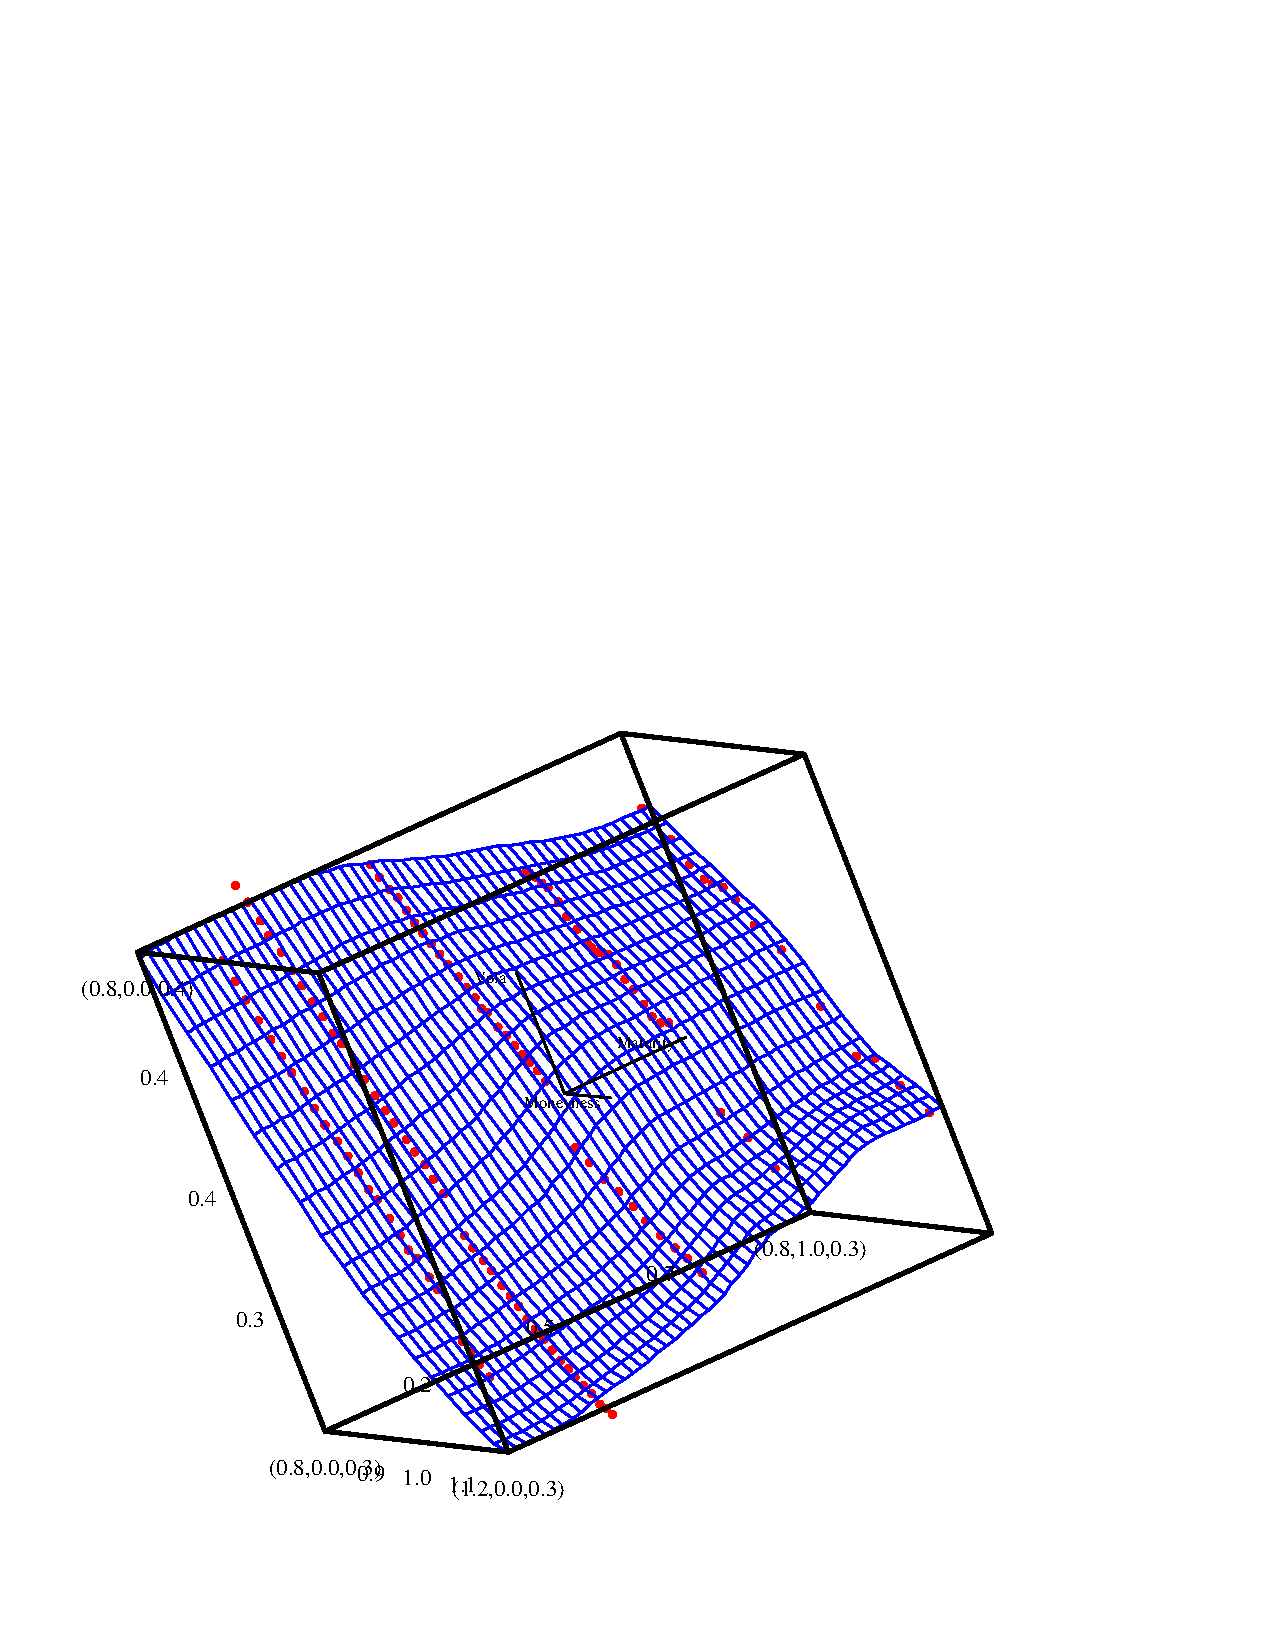
\includegraphics[scale=0.2]{Figures/vola}
			\caption{Include a short, but meaningful caption.}
		\end{center}
	\end{figure}
}

%%%%%%%%%%%%%%%%%%%%%%%%%%%%%%%%%%%%%%%%%%%%%%%%%%%%%%%%%%%%%%%%%%%%%%%%%%%%%%%%%%%%%%%%%%%%%%%%%%%%%%%%%%%%%%%%%%%%%%%%

\frame[containsverbatim]{
	\frametitle{The Package}
	\begin{itemize}
		\item Why we did a package:
		\begin{itemize}
			\item Interface for using funtions
			\item Possibility to share our code
			\item Documentation
		\end{itemize}
		\item How we wrote the package:
		\begin{itemize}
			\item a
			\item b
			\item c
		\end{itemize}
	\end{itemize}
}

%%%%%%%%%%%%%%%%%%%%%%%%%%%%%%%%%%%%%%%%%%%%%%%%%%%%%%%%%%%%%%%%%%%%%%%%%%%%%%%%%%%%%%%%%%%%%%%%%%%%%%%%%%%%%%%%%%%%%%%%

\frame[containsverbatim]{
	\frametitle{Code}
	
	
}

%%%%%%%%%%%%%%%%%%%%%%%%%%%%%%%%%%%%%%%%%%%%%%%%%%%%%%%%%%%%%%%%%%%%%%%%%%%%%%%%%%%%%%%%%%%%%%%%%%%%%%%%%%%%%%%%%%%%%%%%

\frame[containsverbatim]{
	\frametitle{Thank you for your attention!}
	\begin{itemize}
		\item Any remaining questions?
	\end{itemize}
}

% Define the end of the document:
\end{document}
